%%%%%%%%%%%%%%%%%%%%%%%%%%%%%%%%%%%%%%%%%
% Stylish Article
% LaTeX Template
% Version 2.1 (1/10/15)
%
% This template has been downloaded from:
% http://www.LaTeXTemplates.com
%
% Original author:
% Mathias Legrand (legrand.mathias@gmail.com) 
% With extensive modifications by:
% Vel (vel@latextemplates.com)
%
% License:
% CC BY-NC-SA 3.0 (http://creativecommons.org/licenses/by-nc-sa/3.0/)
%
%%%%%%%%%%%%%%%%%%%%%%%%%%%%%%%%%%%%%%%%%

%----------------------------------------------------------------------------------------
%	PACKAGES AND OTHER DOCUMENT CONFIGURATIONS
%----------------------------------------------------------------------------------------

\documentclass[fleqn,10pt]{SelfArx} % Document font size and equations flushed left

\usepackage[english]{babel} % Specify a different language here - english by default

\usepackage{lipsum} % Required to insert dummy text. To be removed otherwise

%----------------------------------------------------------------------------------------
%	COLUMNS
%----------------------------------------------------------------------------------------

\setlength{\columnsep}{0.55cm} % Distance between the two columns of text
\setlength{\fboxrule}{0.75pt} % Width of the border around the abstract

%----------------------------------------------------------------------------------------
%	COLORS
%----------------------------------------------------------------------------------------

\definecolor{color1}{RGB}{0,0,90} % Color of the article title and sections
\definecolor{color2}{RGB}{0,20,20} % Color of the boxes behind the abstract and headings

%----------------------------------------------------------------------------------------
%	HYPERLINKS
%----------------------------------------------------------------------------------------

\usepackage{hyperref} % Required for hyperlinks
\hypersetup{hidelinks,colorlinks,breaklinks=true,urlcolor=color2,citecolor=color1,linkcolor=color1,bookmarksopen=false,pdftitle={Title},pdfauthor={Author}}

%----------------------------------------------------------------------------------------
%	ARTICLE INFORMATION
%----------------------------------------------------------------------------------------

\JournalInfo{Crayon AI CoE VIE, Experience paper APS, 2020 \\ Experience Sharing} % Journal information
\Archive{} % Additional notes (e.g. copyright, DOI, review/research article)

\PaperTitle{Advanced Planning and Scheduling using AI \\ Experience Sharing} % Article title

\Authors{Sebastian Knigge\textsuperscript{1}*, Gerald Podloucka\textsuperscript{2}} % Authors
\affiliation{\textsuperscript{1}\textit{AI Advisor at Crayon, AI CoE Vienna}} % Author affiliation
\affiliation{\textsuperscript{2}\textit{Key Account Manager at Crayon, Crayon Austria}} % Author affiliation
\affiliation{*\textbf{Corresponding author}: sebastian.knigge@crayon.com} % Corresponding author

\Keywords{APS --- ML/AI --- Warehousing --- Advanced Planning} % Keywords - if you don't want any simply remove all the text between the curly brackets
\newcommand{\keywordname}{Keywords} % Defines the keywords heading name

%----------------------------------------------------------------------------------------
%	ABSTRACT
%----------------------------------------------------------------------------------------

\Abstract{Crayon is able to improve certain APS features and deploy it either within an ERP system, or as standalone solution. We have shown that we can rethink entire systems and adjust it from an outcome and user perspective. Possible improvements are: Demand forecasting, Stock Forecasting and Planning under uncertainty. These topics are in the expertise of Crayons AI CoE VIE.}

%----------------------------------------------------------------------------------------

\begin{document}

\flushbottom % Makes all text pages the same height

\maketitle % Print the title and abstract box

\tableofcontents % Print the contents section

\thispagestyle{empty} % Removes page numbering from the first page

%----------------------------------------------------------------------------------------
%	ARTICLE CONTENTS
%----------------------------------------------------------------------------------------

\section*{Introduction} % The \section*{} command stops section numbering

\addcontentsline{toc}{section}{Introduction} % Adds this section to the table of contents

The key enabler of AI is a robust data foundation to train models on, and so it is not surprising that internet companies, which are, by definition, data collectors, were the first to adopt this technology. Whereas private user data is comparably cheap, collecting data in manufacturing tends to be more complicated. Especially connecting product and sensor data is still a big challenge. So, it is not surprising it took the manufacturing and trade sector years to build up the right big-data foundation, which was established in tech overnight. 
As the industry made progress in data collection processes, companies were able to gain value by using this data for Business Intelligence. BI and visualization tools provide rich information to the experts working in warehouses and the shop floor. Still, companies are heavily reliant on industry experts to evaluate information, make decisions upon multiple factors, and monitor processes, to name a few of their tasks. It is time to move to the next level with tools that provide not only information but also directly help operators and experts in decision-making by using AI in manufacturing and warehousing.


%------------------------------------------------

\section{Special Requirements}

\begin{figure*}[ht]\centering % Using \begin{figure*} makes the figure take up the entire width of the page
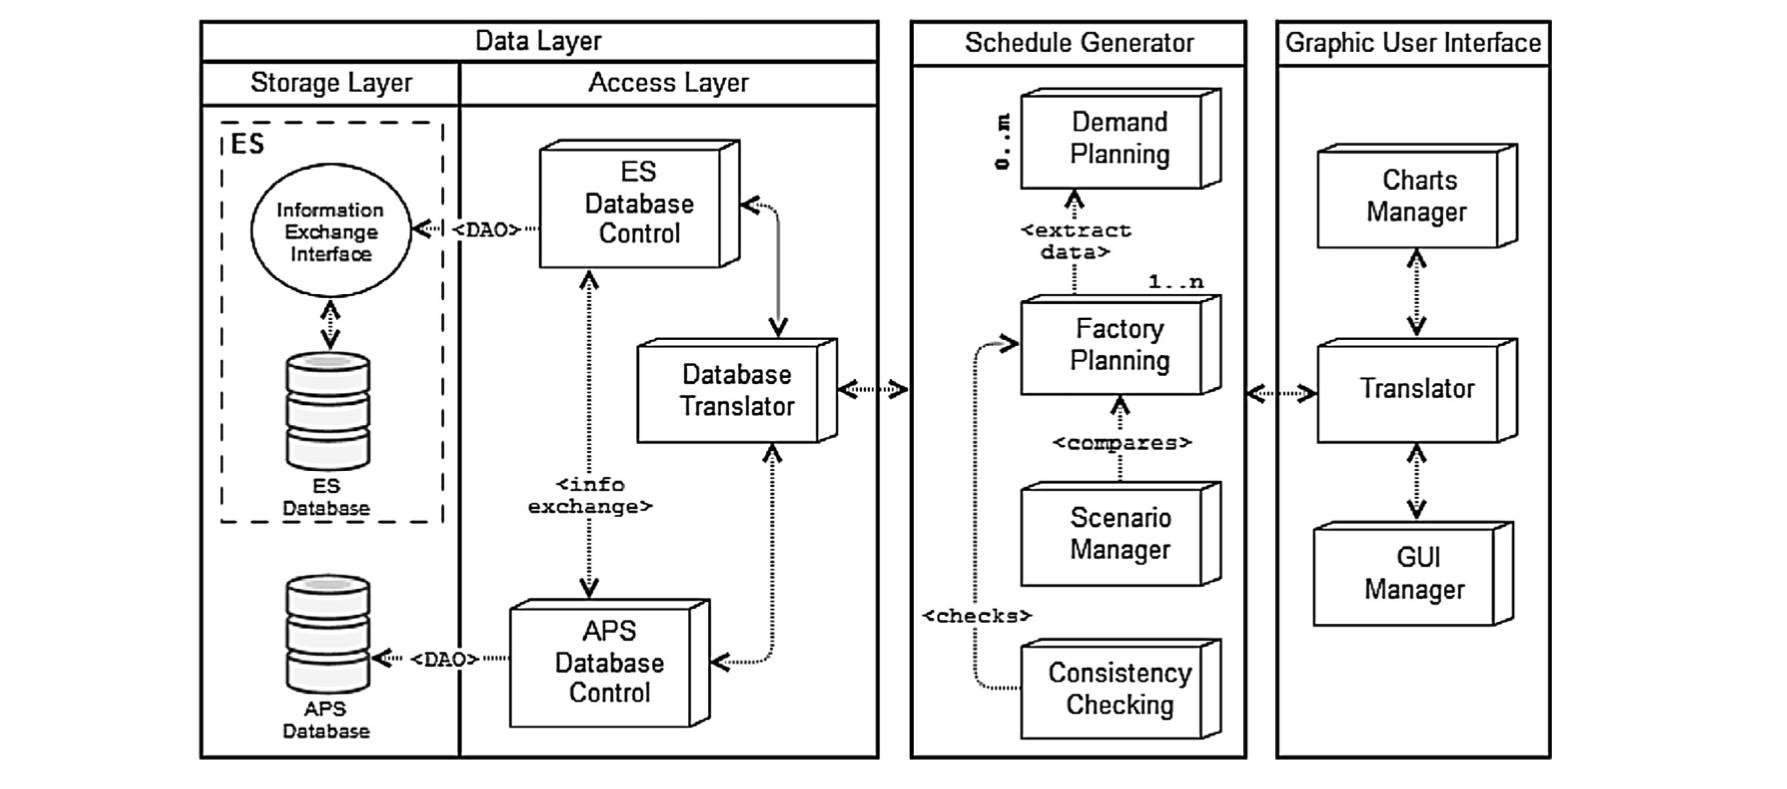
\includegraphics[width=\linewidth]{architecture}
\caption{Sample architecture of generic n-layered mode according to \cite{vidoni2015}}
\label{fig:view}
\end{figure*}

After years of successful delivery for the industry, it is clear to us that delivering solutions tailored to the needs of the companies is the way to go, instead of trying to adjust internal processes to existing off-the-shelf AI tools. We see that solutions are precise to each industry and application area. Also, because of the data available to train the algorithms, most solutions are unique. When we worked together with voestalpine solving very specific business problems in warehouse optimization for the steel industry, our approach was proven. 
While warehouse optimization for private consumer goods is still a reasonably generic problem, the problems in the steel industry for business customers is a niche application and the business is dealing with different requirement:
\begin{itemize}
  \item Heavy parts require considering transportation costs within warehouses
  \item Size differences (massive as well as small) in piece size come with certain restrictions in shipping
  \item Customers are more sensitive to product specifications then they are to price – thus it is reasonable to ignore prices but rely on product specifications
  \item Due to special assumptions customer distributions and ordering behavior is very different from private customers (see Figure \ref{customer_demand})
\end{itemize}


\begin{figure}[ht]\centering
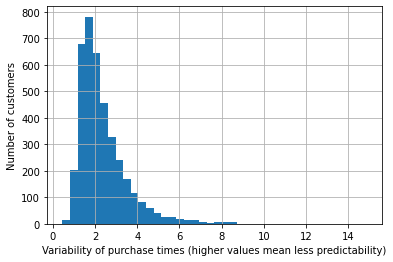
\includegraphics[width=\linewidth]{purchasing_dsitribution.png}
\caption{Example: How regular is the purchase of a given type of piece by a particular party? On average, periods between purchases present a distribution with a std approx. 2x their mean
which means that purchases are not regular and demand at this level of granularity is quite hard to predict.}
\label{customer_demand}
\end{figure}

If one takes these differences into account, techniques from warehouse optimization and other AI applications in customer good (B2C) warehouses can be reused for industries like manufacturing.



\section{APS}

Advanced Planning and Scheduling Systems (APS) or just Advanced Planning Systems are software solutions to visualize information, reduce planning times and allow the simple application of optimization procedures. APS is considered as a supplement to existing ERP systems (often integrated as a separate module) and handles the planning tasks, while the operative transactions remain with the ERP system. \cite{ Stadtler2014}
The three main requirements acc. to \cite{Fleischmann2008} for APS are:
\begin{enumerate}
	\item Holistic planning of the entire supply chain
	\item Convincing optimization through the precise definition of alternatives, goals and constraints of the various planning problems
	\item Hierarchical planning system, which represents a compromise between practicability and the consideration of dependencies between the different planning tasks
\end{enumerate}

\begin{table}[hbt]
\caption{Table of most common ASP Products\\
\scriptsize{Note 1: monday.com is a Production Management software, simplifies production scheduling with real-time tracking for the entire production process to identify bottlenecks, unnecessary delays and unexpected costs at any time; Note 2: FactoryTalk understands physical asset \& digital system performance through 1 consolidated info source. Includes assets inside \& outside the plant; Note 3: Manufacturing Workbench Real-time planning and simulation at any time Cross-plant SCM planning - SAP integration}}
\centering
\begin{tabular}{llr}
\toprule
\multicolumn{2}{c}{Solution} \\
\cmidrule(r){1-2}
Supplier & Product & Note \\
\midrule
monday    & monday.com & Note 1 \\
Aegis & FactoryLogix \\
Katana MRP & Katana \\
Rockwell Automation & FactoryTalk & Note 2 \\
Asprova AG                              & Asprova  \\
ORSOFT         & Manufacturing Workbench  & Note 3\\
\bottomrule
\end{tabular}
\label{suppliers}
\end{table}

See a sample architecture for a APS application in Figure \ref{fig:view}, according to \cite{vidoni2015}.


\subsection{APS Customization}
The advantages of Crayon's AI services definitely reside in the customization of the applications and rethinking business procedures from the user’s perspective. Standard tools are sufficient in some areas to map the basic processes or collect parts of the data. When it comes to the application to a specific case or business, companies almost always use a workaround via Excel to map other data sources or make customized queries (even if they use a specific ERP module). This causes miscalculations and errors in many cases.

\subsection{How Crayons AI will improve prediction} 
There is massive room for improvement in the prediction and forecasting features of APS tools. There are many of the shelve solutions on the market, which are very generic when it comes to the forecasting. Crayons AI CoE VIE is adjusting prediction in following way
\begin{itemize}
  \item \textbf{Demand forecasting}: Demand can be forecasted from previous demand in a time series setting. I.e. only considering one time series which is the one of previous demand and detecting seasonal patterns and general trends. In some cases, it makes sense to use several time series (supply or weather data) to include more information in the model. Still, this are generic models which are not adjusted to the actual business and it’s data, thus special patterns for the demand of some clients are not considered. We could see this in many projects of ours. The algorithm must be trained under certain assumptions of the client (E.g. is negative demand possible?)
  \item	\textbf{Stock Forecasting}: Warehouse or stock is very related to the demand, since there is a direct relation. So predicting stock is not only univariate time series forecasting but multiple time series forecasting under very specific limitations. Some software products include a generic algorithm, but we could see from our experience with voestalpine for example, that standard tools are not applicable for the stock prediction. Sometimes products have very specific inter product correlations and dependencies which standard forecasting does not account for. In such cases, the forecasting is completely worthless and the supply chain team had to estimate by hand. 
\end{itemize}


\subsection{Planning under uncertainty}

The outcome and effect of plans are not certain. Almost all problems involve decision making under uncertainty—that is, choosing actions based on often imperfect observations, with unknown outcomes. Decision Making Under Uncertainty unifies research from different communities using consistent notation and is accessible to students and researchers across engineering disciplines who have some prior exposure to probability theory and calculus \cite{kochenderfer_amato_2015}.
These problems can be approached by classical statistical modelling, using Bayesian networks, decision graphs or even deep learning like reinforcement learning. Which model will be applied to the actual case depends very much on the data. E.g. if there is big data available reinforcement learning is possible, if less data is available or missing data is available, Crayons AI CoE VIE suggests Bayesian networks in case there is some information regarding the dependencies. In any other case we recommend classical statistical modeling, just as we were implementing for voestalpine. See also Figure \ref{models}.

\begin{figure}[ht]\centering
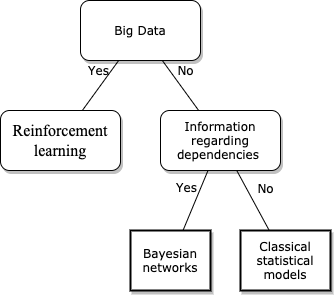
\includegraphics[width=\linewidth]{modeldecision.png}
\caption{Decision diagram to choose modelling approach for decisions under uncertainty}
\label{models}
\end{figure}




%------------------------------------------------

\section{Results and Outlook}

Crayon is able to improve certain APS features and deploy it either within an ERP system, or as standalone solution. We have shown that we can rethink entire systems and adjust it from an outcome and user perspective. Possible improvements are: Demand forecasting, Stock Forecasting and Planning under uncertainty. These topics are in the expertise of Crayons AI CoE VIE.

\subsection{Outlook}

In the future, we will see AI playing a key role in manufacturing and warehousing. Fleet, route and travel time optimization, demand forecasting is possible already. Imagine robots loading or unloading pallets, bringing items to the warehouse or searching items on stock. Entire production plants connected via IoT solutions and optimized production planning and decision-making using machine learning. The list is potentially infinite since for every need satisfied by a smart solution, there will arise a need for a new solution. For some players like Amazon and Alibaba, this is partly reality already. The AI journey for most businesses starts with a very specific use case until a level of confidence is reached to reorganize entire processes with the goal, or at least the possibility, to operate fully automated. 

%------------------------------------------------


%----------------------------------------------------------------------------------------
%	REFERENCE LIST
%----------------------------------------------------------------------------------------
\phantomsection
\bibliographystyle{unsrt}
\bibliography{sample}

%----------------------------------------------------------------------------------------

\end{document}